\subsection{Beam momentum analyzer - D5 magnet}
\begin{figure}[htbp]
  \centering
  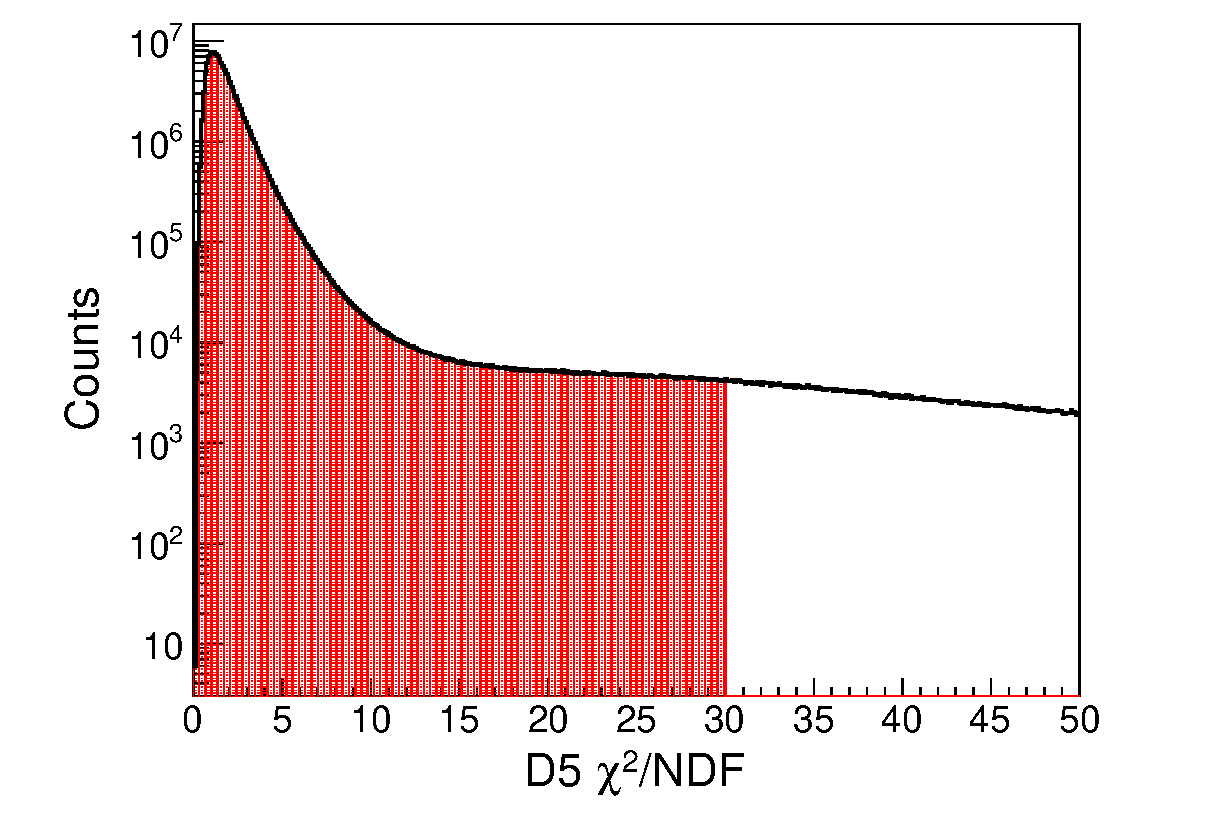
\includegraphics[width=8cm]{../pic/Run78/BL/D5_chi2.eps}
  \caption{
    This figure shows the connected trajectory of BLC1 and BLC2 using the D5 transfer matrix.
    The red hatched region represents an acceptable region.
  }
  \label{fig:D5_chi2}
\end{figure}
\begin{figure}[htbp]
  \begin{tabular}{cc}
    \begin{minipage}{0.5\hsize}
      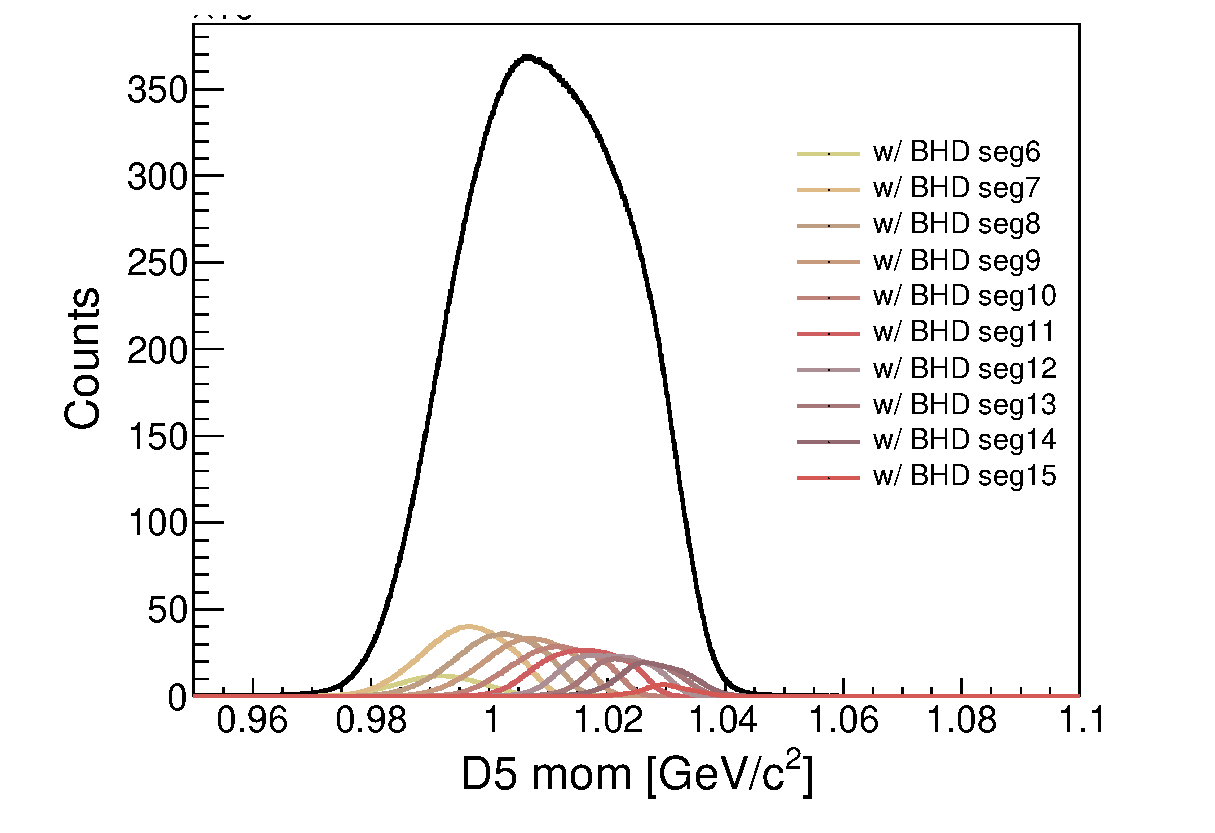
\includegraphics[width=5cm]{../pic/Run78/BL/D5_mom.eps}
    \end{minipage}

    \begin{minipage}{0.5\hsize}
      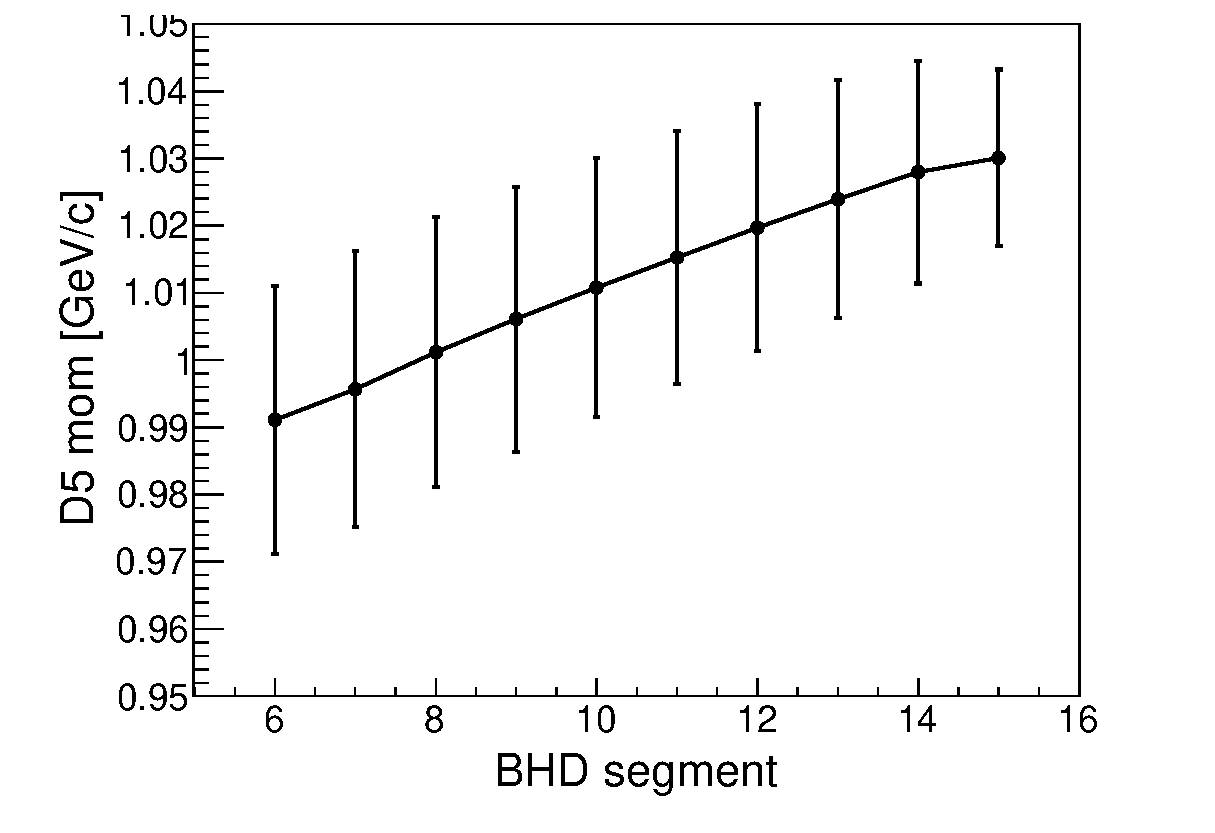
\includegraphics[width=5cm]{../pic/Run78/BL/D5_mom_BHDseg.eps}
    \end{minipage}
  \end{tabular}
  \caption{
    The left figure shows beam momentum. color plots indicate distributions tagged the BHD segment in BHD multiplicity one event.
    The right figure represents center value of momentum as points and matching region as bars.
  }
  \label{fig:D5_BHD}
\end{figure}
Beam particle momentum was calculated by connecting the BLC1 track and the BLC2 track using the transfer matrix of the D5 magnet.
The $\chi^2/NDF$ of connection trajectory was shown as Fig\ref{fig:D5_chi2}. We accept $\chi^2/NDF<30$ events.
Calculated beam momentum distribution is shown as Fig\ref{fig:D5_BHD}, which is seen in the relation between beam momentum and BHD segments.
So, we require 3$\sigma$ level matching between beam momentum and BHD segment, which is shown as the right figure.
